% !TeX spellcheck = fr_FR
\chapter{Chapitre 6 : Détection des problèmes}

\noindent Ce chapitre présente un aperçu de la détection des problèmes après l'appariement des arrêts ATLAS avec les nœuds OSM. Nous y décrivons les types de problèmes, expliquons les logiques de priorisation et concluons par une réflexion sur des pistes d'amélioration.

\section{Types de problèmes détectés}
Notre pipeline signale les problèmes au niveau des arrêts consolidés (\texttt{stops}) et les enregistre dans une table normalisée nommée \texttt{problems}. Quatre catégories de problèmes sont actuellement gérées :
\begin{itemize}
  \item \textbf{Problèmes de distance} — une paire ATLAS–OSM appariée est trop éloignée (en mètres).
  \item \textbf{Problèmes de non-appariement} — un arrêt existe dans une source de données (ATLAS ou OSM) sans correspondant plausible à proximité.
  \item \textbf{Problèmes d'attributs} — des conflits de métadonnées sont détectés sur des paires appariées (opérateur, nom officiel, référence locale, UIC).
  \item \textbf{Doublons (informationnels)} — des SLOIDs dupliqués côté ATLAS ou des nœuds OSM dupliqués pour la même plateforme \texttt{(uic\_ref, local\_ref)} sont identifiés ; ces cas sont utiles pour la révision mais ne constituent pas des contradictions en soi.
\end{itemize}

Chaque problème détecté est caractérisé par un \emph{type}, une \emph{solution} optionnelle (pouvant être renseignée ultérieurement via des « solutions persistantes »), et une \textbf{priorité} numérique (de P1, la plus élevée, à P3, la plus basse) afin de guider l'effort de correction.

\section{Nécessité de la priorisation}
Les problèmes détectés sont nombreux et de criticité variable. Par exemple, un écart de 120 mètres pour un arrêt situé dans un pôle d'échanges majeur est plus problématique qu'une légère différence dans le nom d'un opérateur. Les règles de priorisation sont donc conçues pour refléter cette réalité, afin que l'interface web mette en évidence les anomalies les plus importantes en premier.

\section{Méthode d'attribution des priorités}
Nous calculons les priorités par catégorie de problèmes à l'aide de règles simples. Les règles ci-dessous décrivent la logique appliquée, sans entrer dans les détails d'implémentation.

\subsection{Priorisation des problèmes de distance}
Les critères sont moins stricts pour les arrêts du réseau ferroviaire opérés par les CFF. Les priorités sont attribuées comme suit (pour les paires \texttt{matched}) :
\begin{itemize}
  \item \textbf{P1} — opérateur non CFF et distance strictement supérieure à 80 m.
  \item \textbf{P2} — opérateur non CFF et distance entre 25 m et 80 m (inclus à 80 m).
  \item \textbf{P3} — opérateur CFF et distance strictement supérieure à 25 m ; ou, quel que soit l'opérateur, distance entre 15 m et 25 m (inclus à 25 m).
  \item \textbf{Aucun problème} — distance inférieure ou égale à 15 m, ou distance indisponible.
\end{itemize}

\noindent Ces règles s'appliquent aux paires appariées (\texttt{matched}). Les résolutions de problèmes peuvent être rendues \textbf{persistantes} afin d'être réappliquées lors des imports futurs (voir \S~\ref{sec:persist-workflow}).

\subsection{Priorisation des non-appariements}
Principe : un arrêt isolé, sans correspondant à proximité, est considéré comme un problème prioritaire. Pour guider la revue, nous utilisons les paliers suivants, fondés sur la distance au plus proche voisin et, quand c'est pertinent, sur les identifiants (UIC, quais) :
\begin{description}
  \item[Entrée ATLAS uniquement] \hfill\\
  \begin{itemize}
    \item \textbf{P1} — aucun nœud OSM plausible à proximité (aucun voisin ou voisin au-delà de 80 m).
    \item \textbf{P2} — plus proche nœud OSM au-delà de 50 m ; ou incohérences de comptages UIC/quais à proximité.
    \item \textbf{P3} — cas restants (un voisin plausible existe à moins de 50 m, sans autre alerte forte).
  \end{itemize}
  \item[Nœud OSM uniquement] \hfill\\
  \begin{itemize}
    \item \textbf{P1} — aucun arrêt ATLAS partageant le même UIC dans le voisinage.
    \item \textbf{P2} — plus proche arrêt ATLAS au-delà de 50 m ; ou incohérences de comptages UIC/quais.
    \item \textbf{P3} — cas restants (proximité raisonnable sans indice d'incohérence).
  \end{itemize}
\end{description}

\noindent Les distances au plus proche voisin sont calculées à l'aide d'un KD-tree sur des coordonnées sur la sphère unité, une méthode rapide et numériquement stable. Le rayon d'isolement utilisé est de \textbf{50 m} : la distance linéaire \(d\) est convertie en angle en radians par \(r = 2\,\sin\!\big(\frac{d}{2R_\oplus}\big)\), puis on interroge le KD-tree pour vérifier la présence d'au moins un voisin dans ce rayon. Un arrêt est dit \emph{isolé} s'il n'y a aucun voisin.

\subsection{Priorisation des problèmes d'attributs}
Principe : certains champs (UIC, noms officiels) sont des identifiants critiques et ont donc plus de poids que des champs descriptifs ou opérationnels. Les priorités sont attribuées comme suit (uniquement lorsque les valeurs existent des deux côtés) :
\begin{itemize}
  \item \textbf{P1} — \textbf{UIC différent} (correspondance exacte attendue) \emph{ou} \textbf{nom officiel différent} (comparaison insensible à la casse).
  \item \textbf{P2} — \texttt{local\_ref} différent (insensible à la casse).
  \item \textbf{P3} — opérateur différent (insensible à la casse).
  \item \textbf{Aucun problème} — aucune divergence détectée parmi ces champs.
\end{itemize}

\section{Interface de l'application web}
L'interface propose des filtres simples pour permettre un tri rapide :
\begin{itemize}
  \item \textbf{Filtrer par type de problème} : \texttt{distance}, \texttt{unmatched}, \texttt{attributes}, \texttt{duplicates}.
  \item \textbf{Filtrer par priorité} : \texttt{P1}, \texttt{P2}, \texttt{P3}.
  \item \textbf{Trier} : p. ex. distance la plus grande d'abord, ou par ordre alphabétique du nom d'arrêt.
\end{itemize}

Plus de détails dans le chapitre 9.


\section{Statistiques }

\begin{table}[H]
\centering
\caption{Indicateurs clés de la dernière exécution}
\label{tab:chap6_execution_counters}
\small
\begin{tabular}{l r}
\toprule
Métrique & Nombre \\
\midrule
Total des arrêts importés & \textbf{75\,359} \\
Problèmes de distance & \textbf{10\,124} \\
Problèmes de non-appariement & \textbf{30\,396} \\
Problèmes d'attributs & \textbf{14\,896} \\
Entrées avec problèmes multiples & \textbf{5\,204} \\
Entrées saines (aucun problème) & \textbf{22\,464} \\
\midrule
Entrées avec au moins un problème (dérivé) & \textbf{52\,895} \\
\bottomrule
\end{tabular}
\end{table}

\begin{table}[H]
\centering
\caption{Répartition des problèmes par type et priorité}
\label{tab:chap6_problems_by_priority}
\small
\begin{tabular}{l c c c c}
\toprule
Type de problème & P1 & P2 & P3 & Total \\
\midrule
Problèmes de distance & \textbf{1\,171} & \textbf{4\,179} & \textbf{4\,774} & \textbf{10\,124} \\
Non-appariements & \textbf{8\,192} & \textbf{17\,647} & \textbf{4\,557} & \textbf{30\,396} \\
Problèmes d'attributs & \textbf{7\,045} & \textbf{197} & \textbf{7\,654} & \textbf{14\,896} \\
\bottomrule
\end{tabular}
\end{table}

\begin{table}[H]
\centering
\caption{Répartition détaillée des non-appariements}
\label{tab:chap6_unmatched_breakdown}
\small
\begin{tabular}{l r}
\toprule
Catégorie & Nombre \\
\midrule
ATLAS uniquement & \textbf{8\,416} \\
OSM uniquement & \textbf{21\,980} \\
\midrule
Total non-appariements & \textbf{30\,396} \\
\bottomrule
\end{tabular}
\end{table}



\begin{figure}[H]
  \centering
  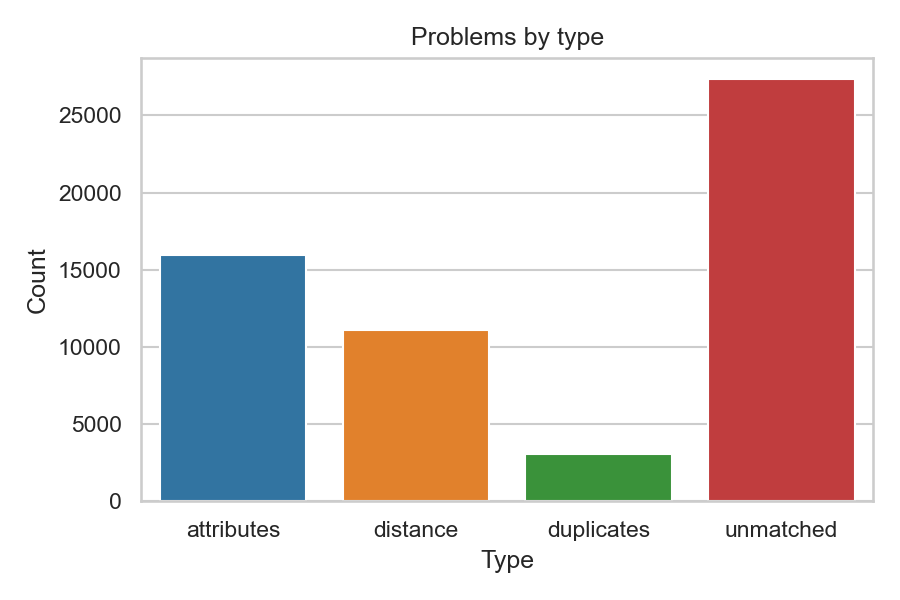
\includegraphics[width=0.85\textwidth]{../figures/chap6/problems_by_type.png}
  \caption[Problèmes par type]{Répartition des problèmes par type.}
\end{figure}

\begin{figure}[H]
  \centering
  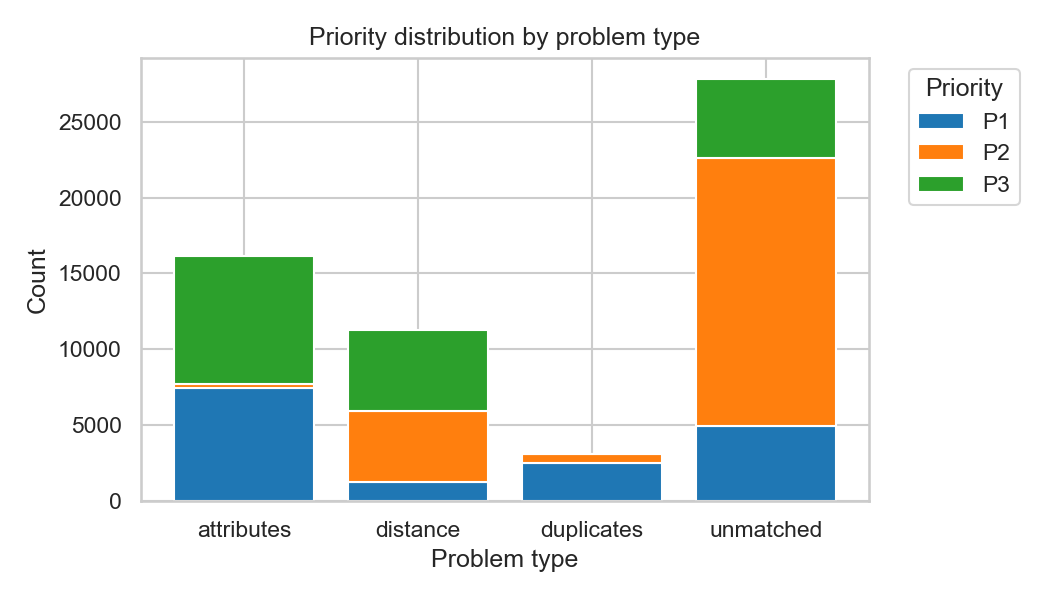
\includegraphics[width=0.85\textwidth]{../figures/chap6/priority_by_type.png}
  \caption[Priorités par type]{Distribution des priorités (P1/P2/P3) par type de problème.}
\end{figure}


\begin{figure}[H]
  \centering
  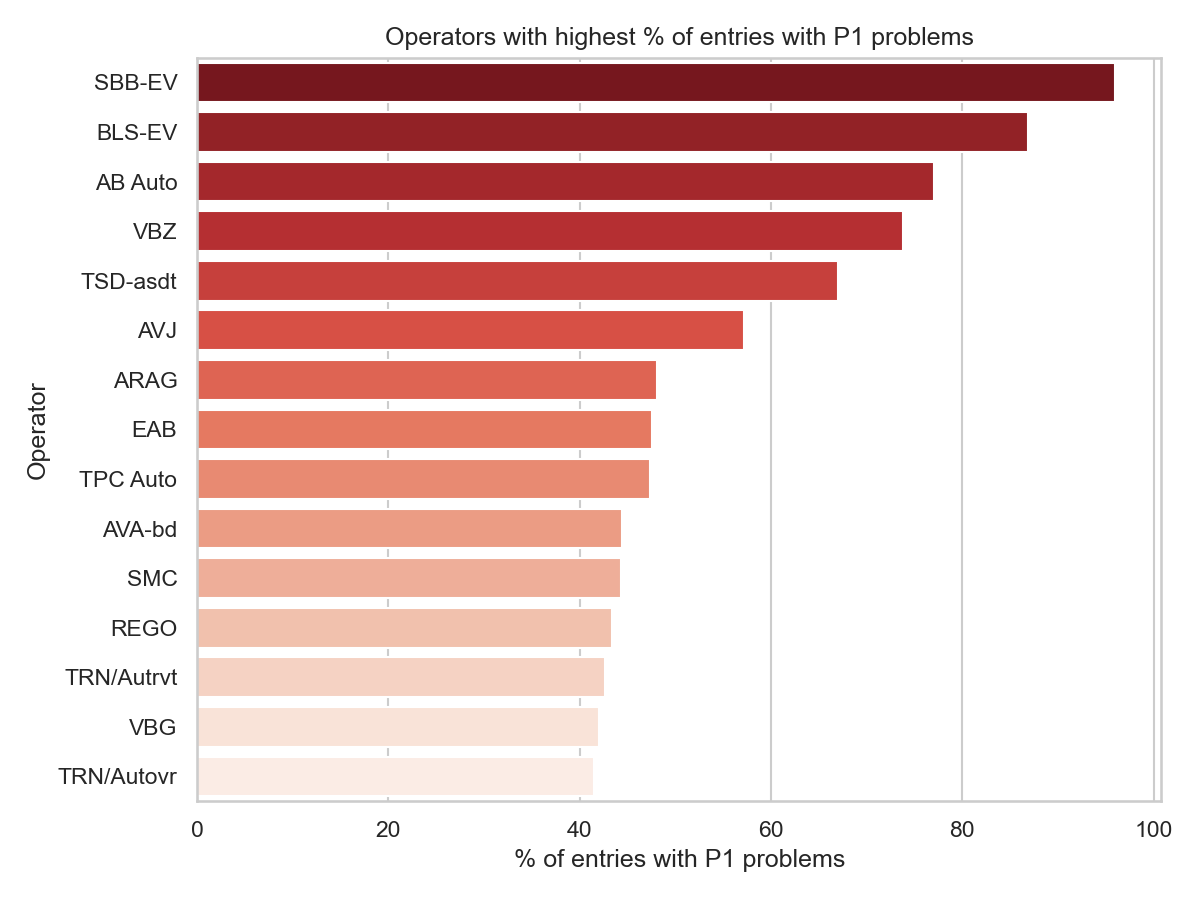
\includegraphics[width=0.85\textwidth]{../figures/chap6/operators_p1_percentage.png}
  \caption[Opérateurs — part des P1]{Opérateurs avec le pourcentage le plus élevé d'entrées présentant des problèmes de priorité P1.}
\end{figure}
\section{Persistance et flux de travail de révision}
\label{sec:persist-workflow}
Deux mécanismes rendent la revue des problèmes efficace dans le temps :
\begin{itemize}
  \item \textbf{Solutions persistantes} — une fois un problème résolu manuellement (p. ex. marqué \texttt{manual} pour un non-appariement), la décision est conservée et réappliquée lors des imports suivants.
  \item \textbf{Notes par côté} — les réviseurs peuvent ajouter des notes ATLAS/OSM qui persistent et s'affichent auprès de l'arrêt.
\end{itemize}

\noindent L'application de ces données persistantes s'effectue à la fin du processus d'import : pour chaque solution enregistrée, les arrêts concernés sont retrouvés, le problème ciblé est mis à jour avec la solution et marqué comme \emph{persistant} afin d'être réappliqué automatiquement lors des prochains imports.
